\documentclass{article}
\usepackage{leonine,amsmath,amssymb,amsthm,graphicx}
\setkeys{Gin}{width=\linewidth,totalheight=\textheight,keepaspectratio}
\graphicspath{{graphics/}}
% Prints a trailing space in a smart way.
% Inserts a blank page
\newcommand{\blankpage}{\newpage\hbox{}\thispagestyle{empty}\newpage}
% \usepackage{units}
% Typesets the font size, leading, and measure in the form of 10/12x26 pc.
\newcommand{\measure}[3]{#1/#2$\times$\unit[#3]{pc}}

\theoremstyle{definition}
\newtheorem{pred}[thm]{Prediction}

\title{Askesis: Granular Cells} \author{Eric Purdy}

\begin{document}

\maketitle


\section{Golgi cells perform non-maximal suppression of the granular cells}

Non-maximal suppression is a special case of a phenomenon called
``explaining away''. When there are two possible causes of a
particular event, knowing that one of the causes did take place lowers
the probability that the other possible cause took place. The classic
example is an alarm that goes off in response to a robbery, but which
can also be set off by an earthquake. Both robbery and earthquake are
very rare events, so their initial probability is low. If all we know
is that the alarm went off, both possible causes become more
likely. If we then learn that an earthquake did indeed take place,
then the probability of a robbery goes back down to something like its
initial probability - the earthquake has ``explained away'' the
evidence provided by the alarm.

Consider now the example of signal coming from muscle spindles, which
fire fastest when their muscle is at a particular length. However,
they also fire more quickly than normal when the muscle is close to
the correct length. Consider two neurons, A, which fires most quickly
when a particular muscle is 12 inches long, and B, which fires most
quickly when the muscle is 13 inches long. If we then learn that both
A and B are firing quickly, but that B is firing more quickly, then
our interpretation should be that the muscle is thirteen inches
long. The firing of A is explained away - it comes from the muscle
being close to the correct length.

We can apply this logic whenever we have two similar events that are
unlikely to hold simultaneously.

In order for the non-maximal suppression performed by the Golgi cell
to make sense, we need to know that the granular cells suppressed by a
particular Golgi cell are similar to one another. Some amount of
similarity is given just by the somatotopic mapping encoded by the
mossy fibers - mossy fibers that are close to one another tend to
respond to stimuli from regions of the body that are close to one
another.

We thus postulate that the granular cells under a particular Golgi
cell function somewhat like a flock of birds: at each time step, each
granular cell updates its parameters to be more correlated with the
Golgi cell, which can be thought of as the center of the flock. The
overall effect is thus to create an ensemble of granular cells to
which non-maximal suppression can be meaningfully applied.

Golgi cells have two kinds of dendrites, basal dendrites which receive
excitatory input from mossy fibers, and apical dendrites which receive
excitatory input from parallel fibers. It has been said \footnote{Eccles et
  al.?}  that the two sets of dendrites are too far apart for the
Golgi cell to perform summation, so we should think of the Golgi cell
as firing when either 1) several nearby mossy fibers are firing, or 2)
many of its parallel fiber inputs are firing.

The Golgi cell also acts to suppress a granular cell that has been
firing for more than a certain amount of time. The granular cell is
active only if it has only recently started firing. Thus its firing
encodes the fact that we have very recently arrived at a very
particular state. The recentness is known because the granular cell
wasn't firing long enough ago to trigger the Golgi cell to suppress
it. The particularity is known because the granular cell is
suppressing all granular cells which are too similar to it but which
are not firing as quickly.

Let $G_i(t)$ be the percentage of the time that the $i$-th granular
cell was firing for a small window of time ending at time $t$. (So,
$G_i(t)=1$ would imply that the $i$-th granular cell is firing at its
maximum rate.) Let $\GGG_i$ be the set of granular cells (excluding
the $i$-th granular cell itself) which receive inhibitory input from
the same Golgi cell as the $i$-th granular cell.  We then have
$$G_i^{nms}(t) = \begin{cases}
1 & G_i(t-1) < \theta \mbox{ and } \forall j\in \GGG_i, G_j(t) < G_i(t)\\
0 & \mbox{otherwise}
\end{cases}, $$
for some threshold $\theta$.

\section{Maximizing the Variance}

Let the $i$-th granular cell's output be defined by
$$G_i(x) = \sigma\left( \sum_j w_{ji} x_j - \theta_i \right).$$

For a fixed mean,
\begin{align*}
Var(G_i) &= \EE_x [ (G_i(x) - \overline{G_i})^2 ] \\
&= \sum_x p(x) (G_i(x) - \overline{G_i})^2 \\
\frac{\partial Var(G_i)}{\partial w_{ji}} &= \sum_x p(x) 2 (G_i(x) - \overline{G_i}) \frac{\partial G_i(x)}{\partial{w_{ji}}}\\
&= \sum_x 2 p(x) (G_i(x) - \overline{G_i}) G_i(x) (1-G_i(x)) x_j\\
\intertext{This leads to the update rule}
\Delta w_{ji} &= \eta G_i(x) (1-G_i(x)) (G_i(x) - \overline{G_i}) x_j,\\
\end{align*}
which yields the BCM rule.

If we allow the mean to vary
\begin{align*}
Var(G_i) &= \EE_x [ (G_i(x) - \overline{G_i})^2 ] \\
&= \sum_x p(x) (G_i(x) - \overline{G_i})^2 \\
\frac{\partial Var(G_i)}{\partial w_{ji}} &= \sum_x p(x) 2 (G_i(x) -
\overline{G_i}) \left[ \frac{\partial G_i(x)}{\partial w_{ji}} -
  \frac{\partial \overline{G_i}}{\partial w_{ji}} \right]\\
&= \sum_x p(x) 2 (G_i(x) -
\overline{G_i}) \left[ G_i(x)(1-G_i(x)) x_j - \sum_y p(y) G_i(y)(1-G_i(y)) y_j \right]\\
&= \sum_x p(x) 2 (G_i(x) -
\overline{G_i}) G_i(x)(1-G_i(x)) x_j \\
&\quad - \sum_x p(x) 2 (G_i(x) - \overline{G_i}) \sum_y p(y) G_i(y)(1-G_i(y)) y_j \\
&= \sum_x p(x) 2 (G_i(x) -
\overline{G_i}) G_i(x)(1-G_i(x)) x_j \\
&\quad - 2 \left(\sum_x p(x) G_i(x) - \sum_x p(x)\overline{G_i} \right) \cdot \left( \sum_y p(y) G_i(y)(1-G_i(y)) y_j \right) \\
\intertext{and this last term vanishes because $\sum_x p(x) G_i(x) =
  \overline{G_i} = \sum_x p(x) \overline{G_i}$. So we end up with the
  same partial derivative, and thus the same update rule.}
\end{align*}



\section{Maximizing the Covariance}
\label{sec-covar}

We wish to derive a learning rule for the mossy fiber-granular cell
synapse that maximizes the covariance between the granular cell and
the Golgi cell which receives and sends feedback to it. This will
create the flocking behavior of the previous section. We actually
modify this desire slightly: we want to maximize the covariance
between the Golgi cell's activity and what the granular cell's
activity {\em would have been} if it received no input from the Golgi
cell\footnote{Actually, having done the calculation both ways (with
  and without input from the Golgi cell), it doesn't make much
  difference. We omit the more complicated case (with the Golgi cell
  input), as it doesn't add much insight.}. The inhibitory input from
the Golgi cell will make the granular cell less correlated with it.

Recall the logistic function $$\sigma(x) = \frac{1}{1 + e^{-x}}.$$
Recall that its derivative is $$\frac{d}{dx}\sigma(x) =
\frac{e^{-x}}{\left(1 + e^{-x} \right)^2} = \sigma(x)(1-\sigma(x)).$$

Consider the situation where we have a number of granular cells which
all excite the same Golgi cell, and which receive inhibitory signals
from that Golgi cell.

Let $x_i$ be a binary variable (either $0$ or $1$) that encodes
whether the $i$-th mossy fiber fired at a particular time step. Let
$x$ be the vector of all the mossy fiber activations, so that $x_i$ is
$1$ exactly when the $i$-th mossy fiber fires, and $0$ otherwise. Let
$p(x)$ be the probability of observing the value $x$. We will assume
that we receive a sample from this distribution at every time step.
In this section, we will assume that each sample is independent of the
others.

Let the $i$-th granular cell's output be defined by
$$G_i(x) = \sigma\left( \sum_j w_{ji} x_j - \theta_i \right).$$
Let the Golgi cell's output be defined by
$$Z(x) = \sigma \left( \alpha \sum_i G_i(x) - \varphi \right).$$
Note that we are assuming that the Golgi cell weights all of its inputs evenly.

As discussed above, we wish to maximize the covariance between $G_i$
and $Z$.  

\begin{align*}
Cov(G_i, Z) &= \EE_x [ G_i(x) Z(x) ] - \EE_x [ G_i(x) ] \EE_y [ Z(y) ] \\
&= \sum_x p(x) G_i(x) Z(x) - \sum_x p(x) G_i(x) \sum_y p(y) Z(y) \\
\frac{\partial Cov(G_i, Z)}{\partial w_{ji}} &= \sum_x p(x) \left[\frac{\partial G_i(x)}{\partial w_{ji}} Z(x) + G_i(x) \frac{\partial Z(x)}{\partial w_{ji}}\right] \\
&\qquad - \sum_x p(x) G_i(x) \sum_y p(y) \frac{\partial Z(y)}{\partial w_{ji}} - \sum_x p(x) \frac{\partial G_i(x)}{\partial w_{ji}} \sum_y p(y) Z(y) \\
\intertext{Letting $\overline{Z} = \sum_y p(y) Z(y)$ and $\overline{G_i} = \sum_x p(x) G_i(x)$, we have}
&= \sum_x p(x) \left[\frac{\partial G_i(x)}{\partial w_{ji}} Z(x) + G_i(x) \frac{\partial Z(x)}{\partial w_{ji}}\right] \\
&\qquad - \overline{G_i} \sum_x p(x) \frac{\partial Z(x)}{\partial w_{ji}} - \overline{Z} \sum_x p(x) \frac{\partial G_i(x)}{\partial w_{ji}} \\
&= \sum_x p(x) \left( Z(x) - \overline{Z}\right) \frac{\partial G_i(x)}{\partial w_{ji}} + \sum_x p(x) \left(G_i(x) - \overline{G_i}\right) \frac{\partial Z(x)}{\partial w_{ji}}
\end{align*}

Now, by the chain rule
\begin{align*}
\frac{\partial G_i(x)}{\partial w_{ji}} &= \sigma' \left(\sum_k w_{ki} x_k - \theta_i\right) \cdot \frac{\partial}{\partial w_{ji}}\left(\sum_k w_{ki} x_k - \theta_i\right)\\
&= G_i(x) (1 - G_i(x)) x_j\\
\intertext{and similarly}
\frac{\partial Z}{\partial w_{ji}}(x) &= Z(x) (1 - Z(x)) \frac{\partial}{\partial w_{ji}} \left(\sum_k \alpha G_k(x) - \phi \right)\\
&= Z(x) (1 - Z(x)) \alpha \frac{\partial G_i(x)}{\partial w_{ji}}\\
&= \alpha Z(x) (1 - Z(x)) G_i(x) (1 - G_i(x)) x_j
\intertext{Substituting this into the above, we arrive at}
\frac{\partial Cov(G_i, Z)}{\partial w_{ji}} &= \sum_x p(x) (Z(x) - \overline{Z}) G_i(x) (1 - G_i(x)) x_j \\
&\qquad + \sum_x p(x) (G_i(x) - \overline{G_i}) \alpha Z(x) (1 - Z(x)) G_i(x) (1 - G_i(x)) x_j \\
&= \sum_x p(x) x_j G_i(x) (1 - G_i(x)) \left[Z(x) - \overline{Z} + \alpha(G_i(x) - \overline{G_i}) Z(x) (1 - Z(x)) \right]\\
&= \alpha \sum_x p(x) x_j G_i(x) (1 - G_i(x)) Z(x) (1 - Z(x)) \left[ G_i(x) - \overline{G_i} + \frac{Z(x) - \overline{Z}}{\alpha Z(x) (1 - Z(x))} \right]\\
\end{align*}

We can use stochastic gradient descent to maximize the covariance,
yielding the update rule
$$\Delta w_{ji} = \eta \alpha x_j G_i(x) (1 - G_i(x)) Z(x) (1 - Z(x)) \left[ G_i(x) - \overline{G_i} + F_\alpha(Z) \right],$$
where $F_\alpha(Z) = \frac{Z - \overline{Z}}{\alpha Z(1 - Z)}$.

For a fixed $Z$, we then have (letting $A = F_\alpha(Z)$)
$$\Delta w_{ji} \propto x_j G_i(x) (1 - G_i(x)) (G_i(x) -
(\overline{G_i} - A)),$$ which yields the BCM rule, with zeros at
$G_i=0, G_i=1$, and $G_i=\overline{G_i}-A$. Note that the middle threshold, where
$\Delta w_{ji}$ switches from negative to positive, varies as a
function of $Z$. Changing $Z$ will thus switch the sign of $\Delta
w_{ji}$ for values of $G$ close to the middle threshold.

\begin{figure}
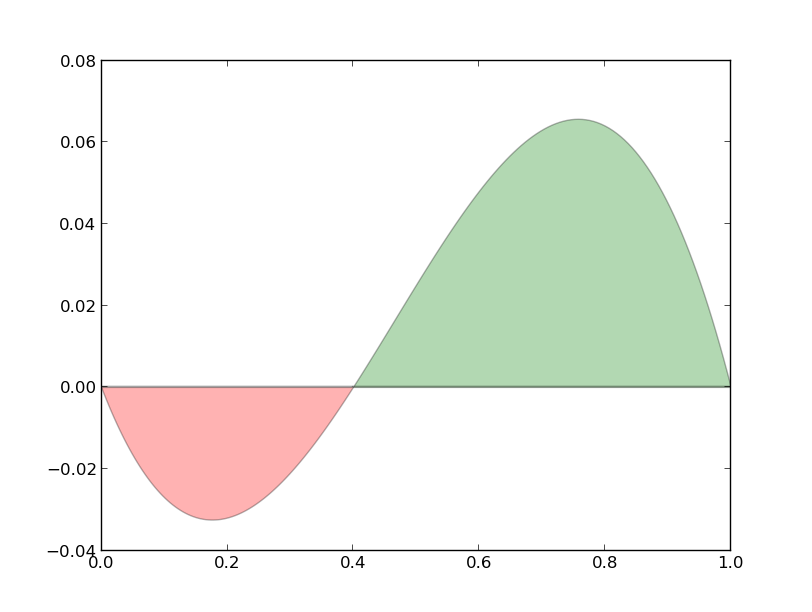
\includegraphics{covar.png}
\caption{$\Delta w_{ji}$ as a function of $G_i$, with $(\overline{G_i} - A) = 0.4$.}
\label{fig-bcm}
\end{figure}

\begin{figure}
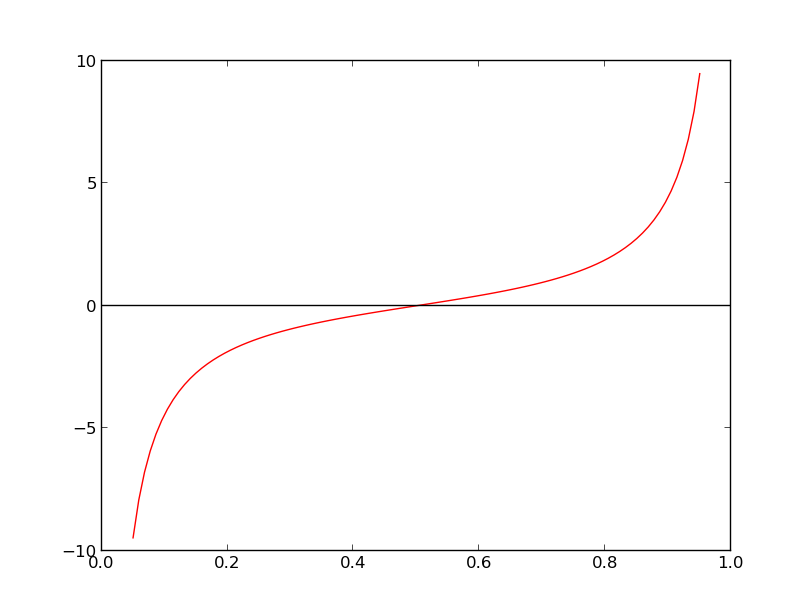
\includegraphics{zgraph.png}
\caption{$F_\alpha(Z) = \frac{Z - \overline{Z}}{\alpha Z(1-Z)}$, with $\overline{Z}
  = 0.5$ and $\alpha=1$}
\label{fig-zgraph}
\end{figure}

\begin{figure}
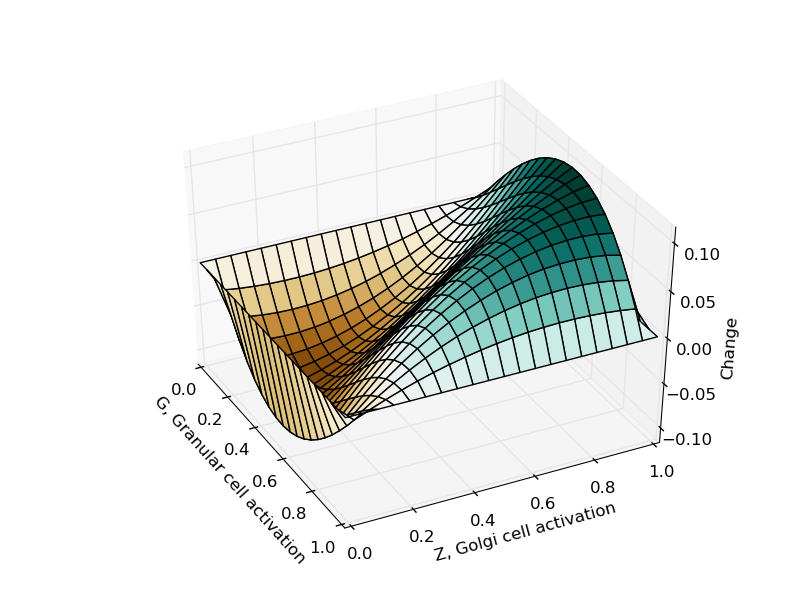
\includegraphics[width=0.5\linewidth]{flocking1.png}
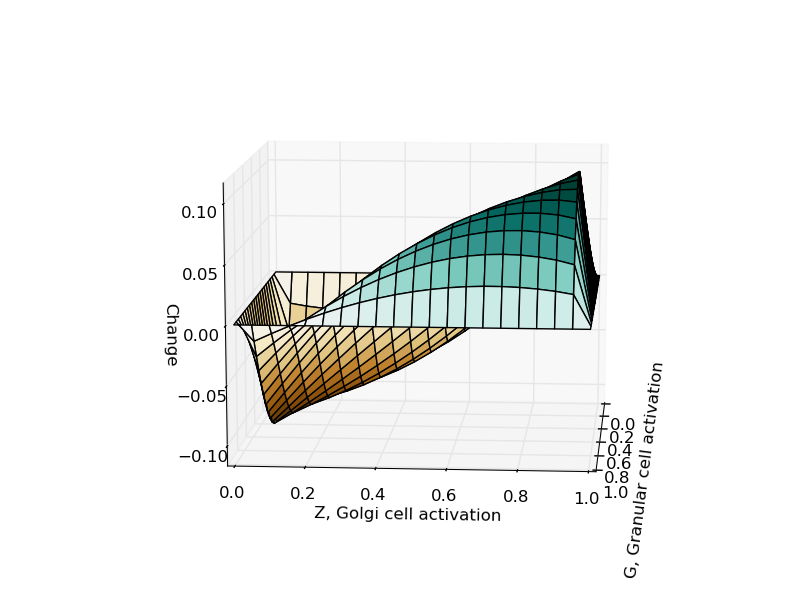
\includegraphics[width=0.5\linewidth]{flocking2.png}
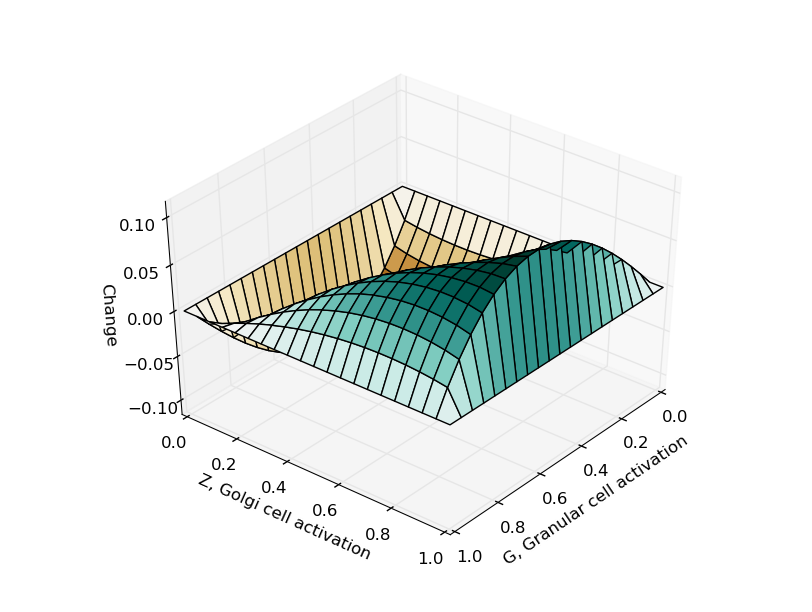
\includegraphics[width=0.5\linewidth]{flocking3.png}
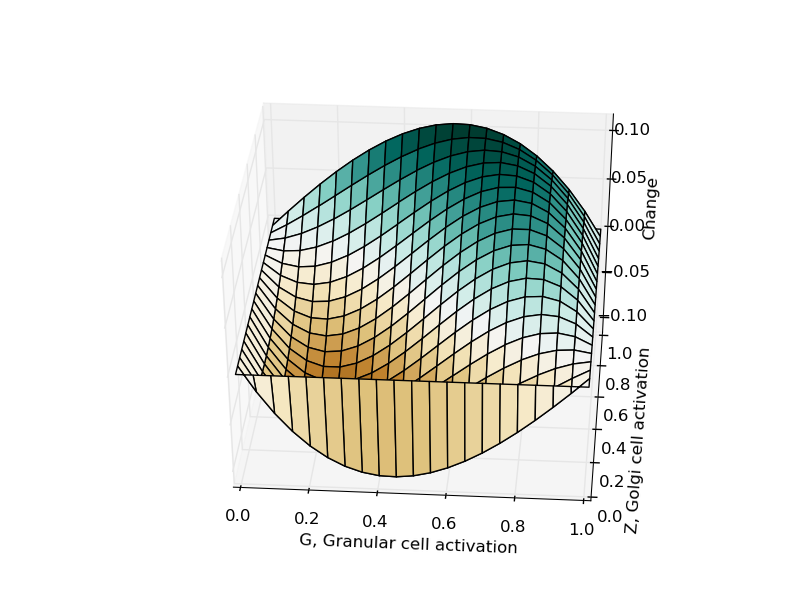
\includegraphics[width=0.5\linewidth]{flocking4.png}
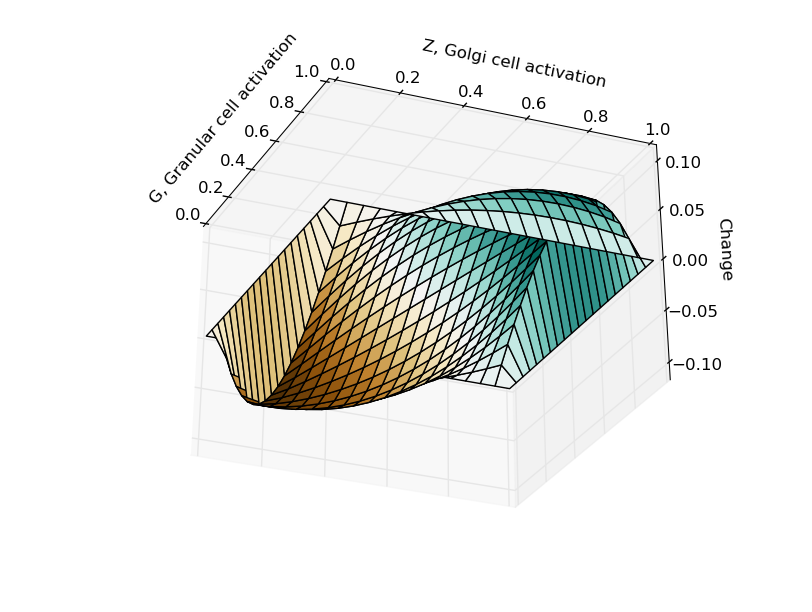
\includegraphics[width=0.5\linewidth]{flocking5.png}
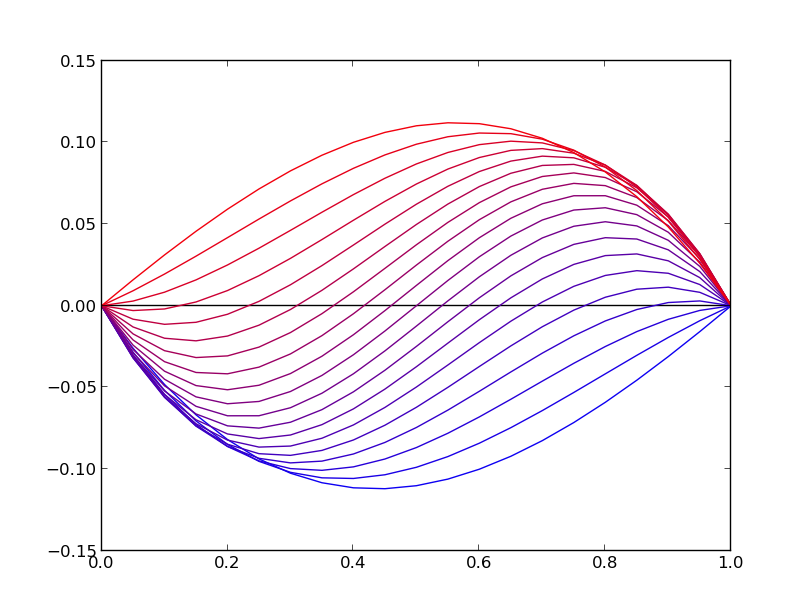
\includegraphics[width=0.5\linewidth]{flocking6.png}
\caption{Change in mossy fiber-granular cell synapse weight as a
  function of Granular cell firing rate ($G$) and Golgi cell firing
  weight ($Z$). The bottom right shows the change as a function of
  $G$; each curve corresponds to one value of $Z$, redder indicating
  higher $Z$, bluer indicating lower $Z$. We are using the parameters
  $\overline{G}=0.5, \overline{Z}=0.5, \alpha=5$.}
\end{figure}

\section{Transition between Update Regimes}

\begin{figure}
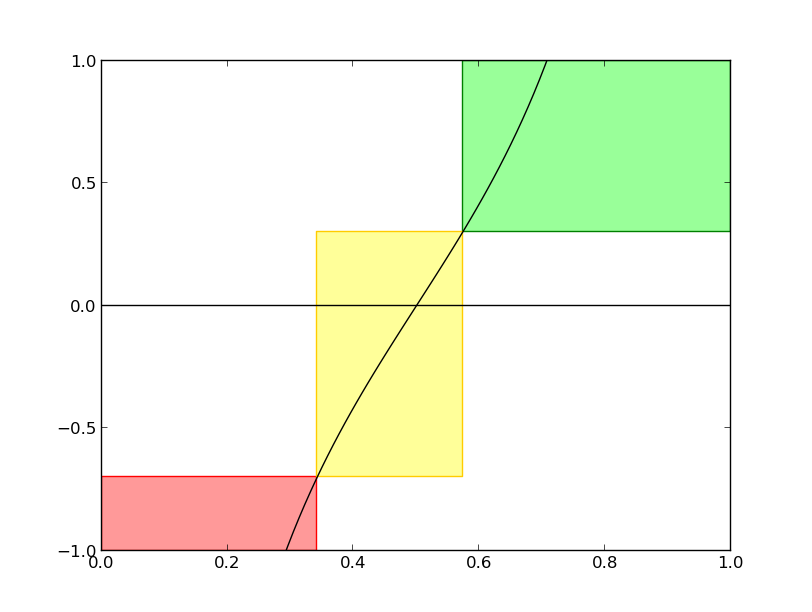
\includegraphics{zgraph2.png}
\caption{The three different regimes: the red box is when $Z$ is low
  and the update is always negative. The green box is when $Z$ is high
  and the update is always positive. The yellow box is when $Z$ is in
  between and the update follows the BCM rule.  With $\overline{Z} = 0.5$,
  $\overline{G_i} = 0.3$, and $\alpha=1$.}
\label{fig-zgraph}
\end{figure}

Recall that our update rule was
$$\Delta w_{ji} = \eta \alpha x_j G_i(x) (1 - G_i(x)) Z(x) (1 - Z(x))
\left[ G_i(x) - \overline{G_i} + F_\alpha(Z) \right],$$ where
$F_\alpha(Z) = \frac{Z - \overline{Z}}{\alpha Z(1 - Z)}$.

There are thus three different regimes:
\begin{enumerate}
\item When $Z$ is sufficiently high, then $(\overline{G_i} -
  F_\alpha(Z))$ is zero or less, and the term $\left[ G_i(x) -
    (\overline{G_i} - F_\alpha(Z)) \right]$ is always positive, so our
  update is always positive.
\item When $Z$ is sufficiently low, then $(\overline{G_i} -
  F_\alpha(Z))$ is more than 1, and the term $\left[ G_i(x) -
    (\overline{G_i} - F_\alpha(Z)) \right]$ is always negative, so our
  update is always negative.
\item When $Z$ is in between, and $(\overline{G_i} - F_\alpha(Z))$ is
  between 0 and 1, we have the BCM rule.
\end{enumerate}

The positive regime starts with $Z$ satisfying
\begin{align*}
\overline{G_i} - F(Z) &= 0\\
%% \overline{G_i} &= \frac{Z-\overline{Z}}{Z(1-Z)} \\
%% \overline{G_i}Z - \overline{G_i}Z^2 &= Z - \overline{Z} \\
%% \overline{G_i}Z^2 + (1-\overline{G_i}) Z -\overline{Z} &= 0\\
\end{align*}
The negative regime starts with $Z$ satisfying
\begin{align*}
\overline{G_i} - F(Z) &= 1\\
%% \overline{G_i} &= 1 + \frac{Z-\overline{Z}}{Z(1-Z)}\\
%% \overline{G_i} &= \frac{Z - Z^2 + Z - \overline{Z}}{Z(1-Z)}\\
%% \overline{G_i}Z - \overline{G_i}Z^2 &= 2Z - Z^2 - \overline{Z}\\
%% (1-\overline{G_i})Z^2 + (\overline{G_i}-2)Z + \overline{Z} &= 0\\
%% \intertext{Using the quadratic formula, the solution to $aZ^2 + bZ + c
%%   = 0$ is $Z = \frac{-b \pm \sqrt{b^2 - 4ac}}{2a}$}
%% Z&= \frac{2 - \overline{G_i} \pm \sqrt{(\overline{G_i}-2)^2 - 4(1-G_i)\overline{Z}}}{2 (1-G_i)}\\
%% Z&= \frac{2 - \overline{G_i} \pm \sqrt{\overline{G_i}^2 -
%%     4\overline{G_i} + 4 - 4\overline{Z} + 4\overline{Z}\overline{G_i}}}{2 (1-G_i)}\\
\end{align*}
Both of these equations can be solved with the quadratic formula, but
we omit the solutions, since they don't shed much light.

\section{Excitability of Granular Cells}

We can also calculate $\frac{\partial Cov(G_i, Z)}{\partial \theta_i}$
to get an update rule for the excitability of the granular cell. We
omit the calculation, as it is analogous to the one above, but the
resulting update rule is:
$$\Delta \theta_i = -\eta G_i(x) (1 - G_i(x)) Z(x) (1 - Z(x)) \left[
  G_i(x) - \overline{G_i} + F_\alpha(Z) \right].$$


Increasing $\theta_i$ makes it harder for the granular cell to fire.
We should expect that low activation of the granular cell leads to
higher $\theta_i$, which leads to less excitability. High activation
of the granular cell should lead to lower $\theta_i$, which leads to
higher excitability. \footnote{This seems like a poor choice.}

Looking at the three regimes:
\begin{enumerate}
\item When $Z$ is high, $G_i - F_\alpha(Z)$ is always zero or less, so
  $\Delta \theta_i$ is always negative, so the granular cell becomes
  more excitable.
\item When $Z$ is low, the granular cell becomes less excitable.
\item When $Z$ is in-between, the sign of the update depends on $G_i$.
\end{enumerate}

\section{Flocking Experiment}

\begin{figure}
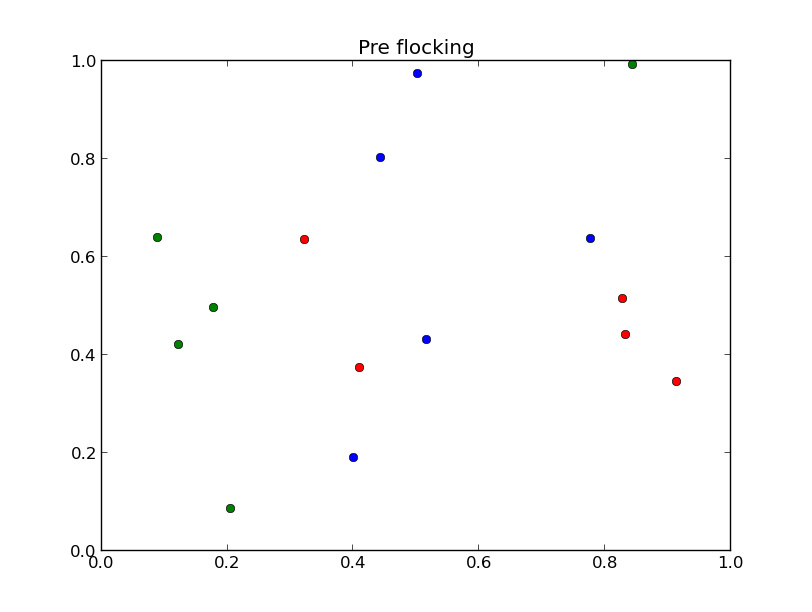
\includegraphics[width=0.5\linewidth]{flock_points_pre1.png}
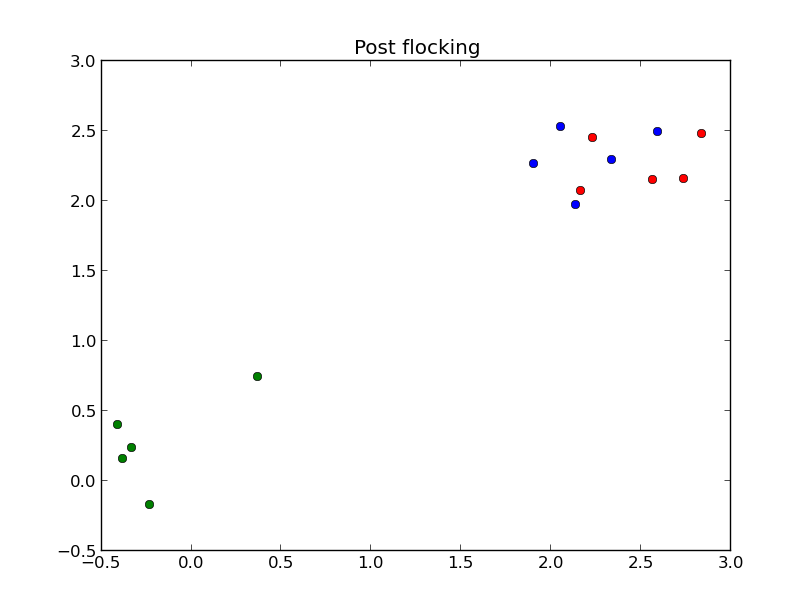
\includegraphics[width=0.5\linewidth]{flock_points_post1.png}
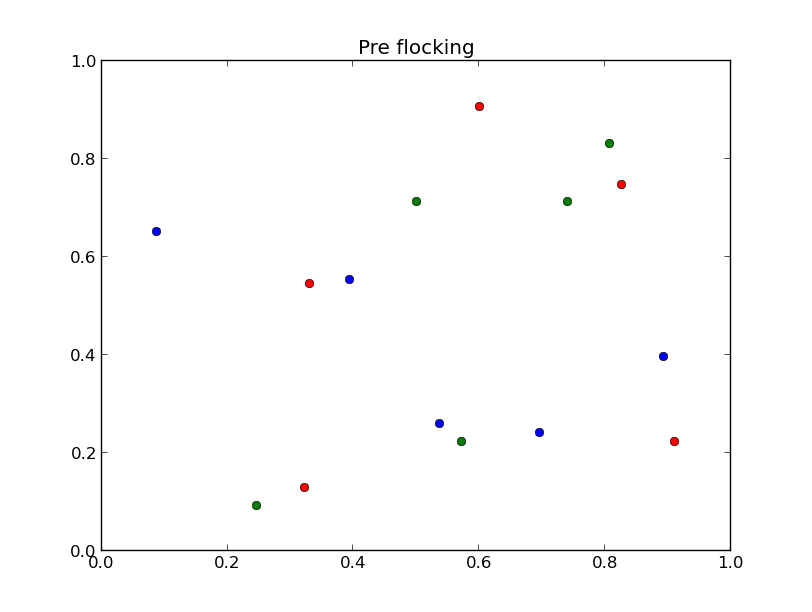
\includegraphics[width=0.5\linewidth]{flock_points_pre2.png}
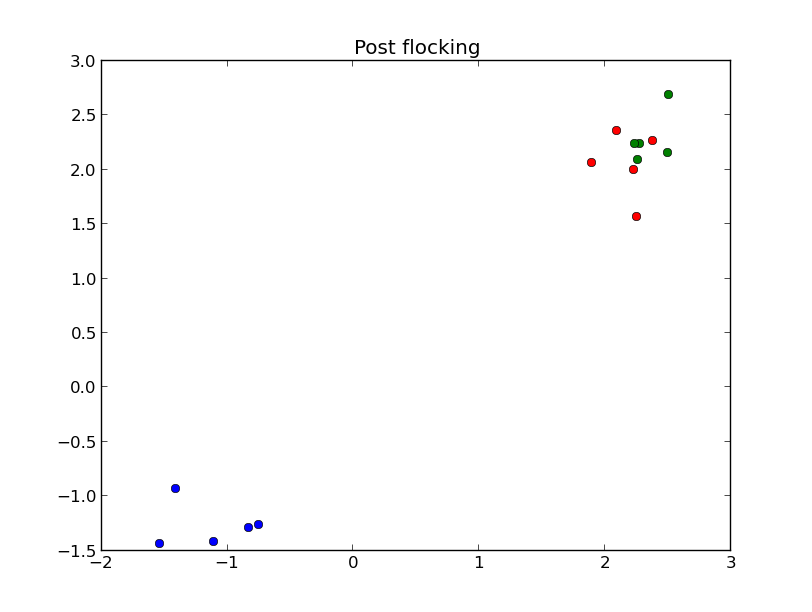
\includegraphics[width=0.5\linewidth]{flock_points_post2.png}
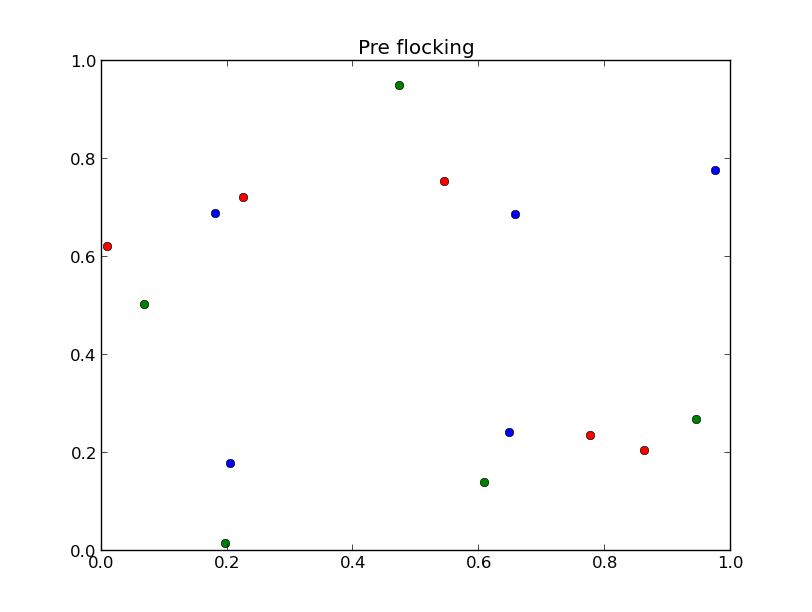
\includegraphics[width=0.5\linewidth]{flock_points_pre3.png}
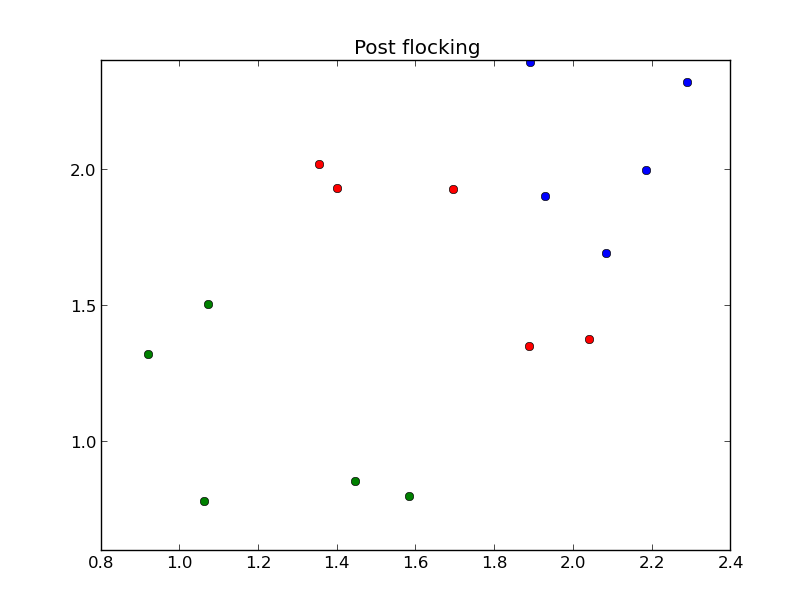
\includegraphics[width=0.5\linewidth]{flock_points_post3.png}
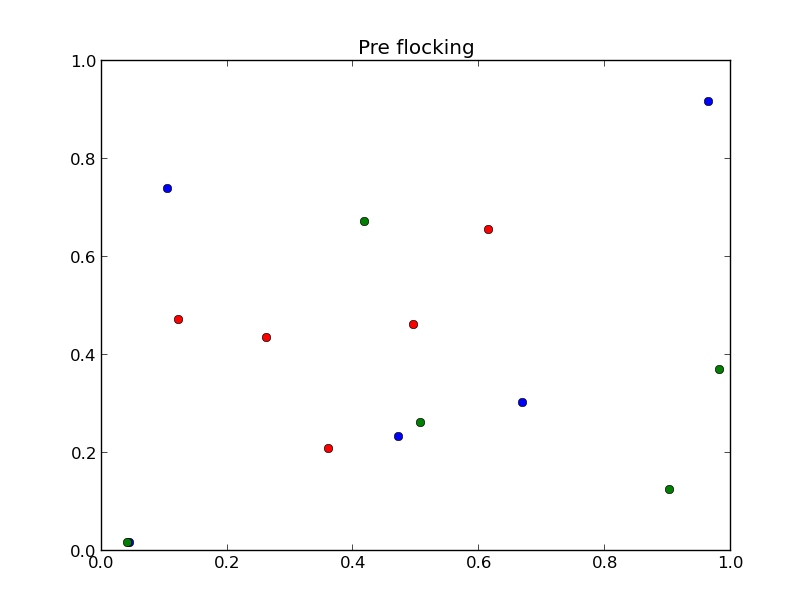
\includegraphics[width=0.5\linewidth]{flock_points_pre4.png}
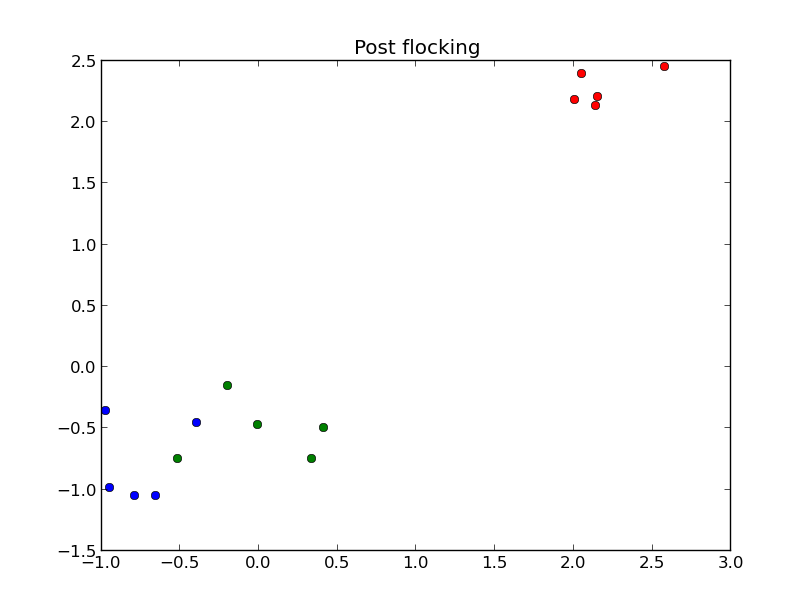
\includegraphics[width=0.5\linewidth]{flock_points_post4.png}\\
\caption{Results of performing flocking on functions of the form
  $G_i=\sigma(ax + by +c)$. Each function is plotted at point $(a,b)$
  for its specific weights $a$ and $b$. The left column shows the
  functions before flocking, the right column the corresponding trial
  after flocking. }
\label{fig-flocking-experiment}
\end{figure}

We conducted some flocking experiments using 15 random functions of
the form
$$G_i=\sigma(ax + by + c).$$ We grouped the points into three groups
(red, green, and blue), and applied the flocking update rule on random
input for 10,000 iterations. The results are shown in Figure
\ref{fig-flocking-experiment}.  Note the randomness of the input and
the similarity of the output. Also note that we often wind up with
overlapping clusters; this is less likely in higher dimensions.



\section{Predictions}

\begin{pred}
Mossy fiber - granular cell synapse should follow a learning rule like
that given above in Section \ref{sec-covar}.
\end{pred}

\begin{pred}
The Purkinje cells that a particular basket or stellate cell
innervates should suppress the same deep nuclear cell. Or, more
weakly, they should suppress deep nuclear cells with similar firing
patterns. This is necessary for the basket/stellate cell to make sense
as the site for negative weights of the corresponding Purkinje cell.
\end{pred}

\begin{pred}
Each Golgi cell should inhibit roughly the same set of granular cells
which excite it. These granular cells should also be excited by the
same set of mossy fibers that excite the Golgi cell. (I think this is
already known to be true, but I'm not sure.) This is necessary for the
granular cells under a particular Golgi cell to make sense as a flock.
\end{pred}

\begin{pred}
If you prevent a Golgi cell from firing, the granular cells it outputs
to should be somewhat correlated in their firing patterns. If you then
allow the Golgi cell to fire, the granular cells should become more
correlated. (This only holds true if the granular cells are being fed
a stream of mossy fiber activations from the same distribution as the
one they learned from.)
\end{pred}

\begin{pred}
Two mossy fiber inputs to a Golgi cell should be more correlated than
two mossy fibers which are the same distance apart but which do not
synapse on the same Golgi cell. This would be the result of following
the flocking rule.
\end{pred}

\begin{pred}
Either the inferior olive receives a copy of the signal from some
command mossy fibers, or the negative pathway does not suppress state
transitions. In the latter case, there should be no active synapses
between Purkinje cells and state cells.
\end{pred}

\begin{pred}
Each inferior olive cell should send a collateral to the same deep
nuclear cell that its Purkinje cell(s) projects to. If this is not the
case, then the two deep nuclear cells (the one receiving the
collateral and the one receiving the output of the Purkinje cell)
should exhibit similar firing patterns. This is necessary for the
inferior olive cell to have a single coherent meaning: that it fires
when we desire to see more firing from the relevant deep nuclear cell.
\end{pred}

\begin{pred}
The mossy fibers of state cells, context cells, and command cells
should be intermingled when they reach the granular cell, so that each
granular cell can potentially form synapses with mossy fibers of all
three types. This increases the representational ability of the
system.
\end{pred}

\end{document}
